% !TEX program = xelatex
\documentclass[fontset=windows, 12pt, a4paper]{ctexart}

\usepackage[a4paper, top=2.5cm, bottom=2.5cm, left=2.5cm, right=2.5cm]{geometry}
\usepackage{amsmath}
\usepackage{graphicx}
\usepackage{float}
\usepackage{booktabs}
\usepackage{array}
\usepackage{xcolor}
\usepackage{listings}

\IfFontExistsTF{Times New Roman}{\setmainfont{Times New Roman}}{}
\IfFontExistsTF{Consolas}{\setmonofont{Consolas}}{}

\linespread{1.43}
\setlength{\parindent}{2em}

\ctexset{
  section/number       = \chinese{section},
  subsection/number    = \arabic{section}.\arabic{subsection},
  subsubsection/number = \arabic{section}.\arabic{subsection}.\arabic{subsubsection},
}

\usepackage{titlesec}
\titleformat{\section}
  {\centering\fontsize{17.3pt}{20.8pt}\heiti\bfseries}
  {\chinese{section}、}{1em}{}
\titleformat{\subsection}
  {\fontsize{14.45pt}{17.4pt}\heiti\bfseries}
  {\arabic{section}.\arabic{subsection}}{1em}{}
\titleformat{\subsubsection}
  {\fontsize{12.05pt}{14.5pt}\heiti\bfseries}
  {\arabic{section}.\arabic{subsection}.\arabic{subsubsection}}{1em}{}
\titlespacing{\section}       {0pt}{1.25em}{0.82em}
\titlespacing{\subsection}    {0pt}{1.15em}{0.55em}
\titlespacing{\subsubsection} {0pt}{1.15em}{0.55em}

\usepackage{tocloft}
\renewcommand{\cftsecfont}{\heiti\bfseries}
\renewcommand{\cftsecpagefont}{\heiti\bfseries}
\renewcommand{\cftsecleader}{\cftdotfill{\cftdotsep}}
\renewcommand{\cftsubsecleader}{\cftdotfill{\cftdotsep}}
\renewcommand{\cftsubsubsecleader}{\cftdotfill{\cftdotsep}}

\lstset{
  basicstyle=\ttfamily\small,
  backgroundcolor=\color{black!3},
  frame=single,
  framesep=6pt,
  rulecolor=\color{black!30},
  framerule=0.8pt,
  breaklines=true,
  showstringspaces=false,
  columns=fullflexible,
  keepspaces=true,
}

\pagestyle{plain}

\newcommand{\papertitle}[1]{%
  \thispagestyle{empty}%
  \begin{center}
    {\fontsize{17.3pt}{22pt}\bfseries #1}
  \end{center}
  \vspace{1em}
}
\newcommand{\abstractcn}[2]{%
  \thispagestyle{empty}%
  \begin{center}{\fontsize{14pt}{17pt}\bfseries 摘要}\end{center}
  #1\par
  \vspace{1em}
  {\heiti\bfseries 关键字：}#2\par
  \newpage
}
\makeatletter
\newcommand{\tocpage}{%
  \setcounter{page}{1}%
  \begin{center}
    {\fontsize{17.3pt}{20.8pt}\heiti\bfseries 目录}
  \end{center}
  \vspace{0.5em}
  \@starttoc{toc}%
  \newpage
}
\makeatother
\newcommand{\referencescn}{%
  \addcontentsline{toc}{section}{参考文献}%
  % 参考文献。一级标题由 main.tex 中的 \referencescn 生成。

\begin{thebibliography}{99}
\bibitem{prob} 全国大学生数学建模竞赛组委会. 2023年高教社杯全国大学生数学建模竞赛B题：多波束测线问题[Z]. 2023.
\bibitem{ref_book} 赵建虎, 刘经南. 多波束测深及图像数据处理[M]. 武汉: 武汉大学出版社, 2008.
\end{thebibliography}
%
}
\newcommand{\appendixcn}{%
  \section*{附录 A\quad 核心代码}%
  \addcontentsline{toc}{section}{附录 A\quad 核心代码}%
  \vspace{0.8em}

完整可运行程序、原始数据和结果工作簿随论文作为支撑材料提交。本附录仅保留文件对应关系、核心计算流程与复现顺序，避免重复打印正文已经解释的公式和大段源代码。

\subsection*{A.1 支撑材料对应关系}

\begin{table}[H]
  \centering
  \caption{四问程序、输入与输出文件}
  \small
  \begin{tabular}{p{0.34\textwidth}p{0.24\textwidth}p{0.30\textwidth}}
    \toprule
    \textbf{程序} & \textbf{主要输入} & \textbf{主要输出} \\
    \midrule
    \texttt{q1\_multibeam\_model.py} & 题面几何参数 & \texttt{result1.xlsx}：水深、覆盖宽度与重叠率 \\
    \texttt{q2\_multibeam\_model.py} & 航向、距离与坡度 & \texttt{result2.xlsx}：任意航向覆盖宽度 \\
    \shortstack[l]{\texttt{q3\_survey\_line\_}\\\texttt{design.py}} & 规则海域及重叠约束 & \texttt{result3.xlsx}：测线坐标与约束复核 \\
    \shortstack[l]{\texttt{q4\_real\_bathymetry\_}\\\texttt{design.py}} & \texttt{附件.xlsx} 水深网格 & \texttt{result4.xlsx}：候选方案、推荐坐标与覆盖评价 \\
    \texttt{make\_figures.py} & 四份结果工作簿 & 11 张候选图，其中正文采用 9 张 \\
    \bottomrule
  \end{tabular}
\end{table}

\subsection*{A.2 四问核心计算流程}

\begin{enumerate}
  \item \textbf{问题一：二维覆盖计算。}读取开角、坡度、中心水深和测线位置；按式~\eqref{eq:q1_depth}计算船位水深，按式~\eqref{eq:q1_half}计算左右水平半覆盖宽度，再由式~\eqref{eq:q1_overlap_width}和式~\eqref{eq:q1_overlap}逐对计算重叠率。程序同时执行平底极限检查并写出表格结果。

  \item \textbf{问题二：任意航向推广。}遍历题面给定的航向角与距中心距离；先计算船位水深和扫描剖面的等效坡度，再调用问题一的覆盖关系得到水平覆盖宽度。输出前检查特殊航向退化关系和方向对称性。

  \item \textbf{问题三：规则海域递推。}使首条南北向测线的西覆盖边界与海域西界相接；其后以 $10\%$ 目标重叠率为条件，通过二分法求下一条测线的最大可行横坐标，直至末条覆盖东界。最后检查首末边界、全部相邻重叠率以及减少一条测线后的东侧缺口。

  \item \textbf{问题四：真实地形分带。}读取并审计 $201\times251$ 水深网格，计算东西向局部梯度；对每个候选带高独立执行边界贴合与无漏测递推，再把全部线段回代原网格，统计总长度、漏测率、超 $20\%$ 重叠长度、最大重叠率和线段数，形成候选方案比较表。
\end{enumerate}

\subsection*{A.3 复现顺序与结果追踪}

依次运行问题一至问题四程序，分别生成对应的四份结果工作簿。随后运行绘图程序生成候选图。论文表~\ref{tab:q1}、表~\ref{tab:q2}、问题三方案指标和表~\ref{tab:q4}分别对应上述四份工作簿。全部程序以米为内部长度单位，读取附件中的海里坐标后统一按 $1$ 海里 $=1852$ 米换算。

为便于独立核验，四份工作簿同时保留方案摘要、逐线或逐段坐标以及约束检查结果；正文只呈现回答题目所必需的汇总值，完整数值明细均可由支撑材料追溯。
%
}

\begin{document}

\papertitle{多波束测线覆盖宽度建模与最短测线优化设计}

\abstractcn{%
本文针对 2023 年高教社杯全国大学生数学建模竞赛 B 题，研究多波束测深系统的覆盖宽度、相邻条带重叠率与测线布设问题。

针对问题一，本文在与测线方向垂直的二维剖面内建立斜坡多波束覆盖的几何模型。以测线位置 $x$ 的水平距离为变量，给出水深 $D(x)=D_0-x\tan\alpha$，由声束边界与坡面交点推导左右半覆盖宽度 $B_L,B_R$ 及覆盖宽度 $W=B_L+B_R$，并以“当前条带宽度”为分母定义相邻条带重叠率 $\eta_i=O_i/W(x_i)$。代入开角 $120^\circ$、坡度 $1.5^\circ$、中心水深 $70\text{ m}$，得到覆盖宽度由 $-800\text{ m}$ 处的 $315.71\text{ m}$ 单调减小至 $800\text{ m}$ 处的 $170.27\text{ m}$，相邻重叠率由 $35.70\%$ 降至 $-12.36\%$，说明浅水侧会出现漏测。模型在 $\alpha=0$ 时退化为平底公式 $W=2D\tan(\theta/2)$，验证了模型正确性。

针对问题二，本文将二维模型推广到三维坡面。通过坡面法向水平投影与测线方向的夹角 $\beta$，给出船位水深 $D(r,\beta)=D_0+s\tan\alpha\cos\beta$ 与垂直测线剖面的等效坡度 $\alpha_{\mathrm{eff}}=\arctan(\tan\alpha\sin\beta)$，再代入二维覆盖宽度公式。结果表明 $\beta=90^\circ,270^\circ$ 时船沿等深线运动、覆盖宽度恒为 $416.55\text{ m}$；$\beta=0^\circ$ 时随距离增加覆盖宽度由 $415.69\text{ m}$ 增至 $768.48\text{ m}$，与深浅方向变化一致。

针对问题三，本文在规则单坡面矩形海域内建立以测线总长度最小为目标、以完全覆盖和 $10\%\sim20\%$ 重叠率为约束的优化问题。采用“沿等深线南北向布设 + 贪心递推”求解，每步取重叠率下限 $10\%$ 以最大化间距，得到 $34$ 条测线，总长度 $125936.00\text{ m}$（$68.00$ 海里）；东西边界均被覆盖且相邻重叠率全部为 $10.00\%$，并验证少一条测线将出现 $25.76\text{ m}$ 缺口，说明在该方向下测线数已不可再减少。

针对问题四，本文利用附件 $201\times251$ 水深网格估计东西向局部坡度，采用南北向分带递推布线和网格覆盖仿真评价。比较全域、$1.00$、$0.50$、$0.25\text{ NM}$ 四种分带方案后，推荐 $0.50\text{ NM}$ 分带方案：测线线段 $461$ 段，总长度 $426886.00\text{ m}$，漏测率为 $0.00\%$，重叠率超过 $20\%$ 的部分总长 $5481.92\text{ m}$，在完全覆盖前提下兼顾了测线长度、冗余与可执行性。%
}{%
多波束测深 \quad 覆盖宽度 \quad 重叠率 \quad 几何建模 \quad 测线优化 \quad 递推布线%
}

\tocpage

\section{问题重述}

\subsection{问题背景}

单波束测深利用声波在海水中的匀速直线传播测量垂直水深，其测深数据沿航迹密集、测线间缺失。多波束测深系统在与航迹垂直的平面内一次发射多个波束，在海底平坦海域能形成以测线为轴、具有一定宽度的全覆盖水深条带。条带的覆盖宽度 $W$ 随换能器开角 $\theta$ 和水深 $D$ 变化；相邻平行条带的重叠率定义为 $\eta=1-d/W$，其中 $d$ 为相邻测线间距，$\eta<0$ 表示漏测。为保证数据完整，相邻条带通常要求 $10\%\sim20\%$ 的重叠率。真实海底起伏较大，若按平均水深或最浅处水深固定布设测线，会在浅水处漏测或深水处冗余。本文研究对象与任务均来自竞赛题面\cite{prob}。

\subsection{问题内容}

\textbf{问题一：}在与测线方向垂直的平面内，海底坡面与水平面夹角为 $\alpha$。建立多波束覆盖宽度及相邻条带重叠率的数学模型；当开角为 $120^\circ$、坡度为 $1.5^\circ$、中心水深为 $70\text{ m}$ 时，计算表 1 所列位置的指标并保存至 \texttt{result1.xlsx}。

\textbf{问题二：}考虑矩形待测海域，测线方向与海底坡面法向在水平面投影的夹角为 $\beta$，建立覆盖宽度模型；当开角为 $120^\circ$、坡度为 $1.5^\circ$、中心水深为 $120\text{ m}$ 时，计算表 2 所列位置与方向下的覆盖宽度并保存至 \texttt{result2.xlsx}。

\textbf{问题三：}在南北长 $2$ 海里、东西宽 $4$ 海里的矩形海域内，中心水深 $110\text{ m}$、西深东浅、坡度 $1.5^\circ$、开角 $120^\circ$。设计一组总长度最短、完全覆盖且相邻重叠率满足 $10\%\sim20\%$ 的测线。

\textbf{问题四：}附件 \texttt{附件.xlsx} 为某海域（南北 $5$ 海里、东西 $4$ 海里）的单波束测深数据。设计多波束测线，使条带尽可能覆盖整个海域、相邻重叠率尽量不超过 $20\%$、测线总长度尽可能短，并计算测线总长度、漏测面积占比与重叠率超过 $20\%$ 部分的总长度。

\section{问题分析}

\subsection{总体分析}

四个子问题围绕“覆盖宽度”与“测线布设”两个主题层层递进：问题一建立二维剖面的基础几何模型，问题二将其推广到三维坡面，问题三在规则坡面海域上做最短测线优化，问题四进一步面向真实水深网格做数据驱动的分带布线。各问的覆盖宽度模型保持一致口径，即水平投影覆盖宽度，从而可与水平测线间距直接比较。

\subsection{问题一的分析}

问题一的核心是由换能器开角、坡度和测线位置确定单个条带的覆盖宽度及相邻条带的重叠率。由于题目给定的是理想斜坡剖面，所有参数已知，本问本质是二维几何建模与确定性计算。测线两侧的声束与坡面的交点不对称，左右半覆盖宽度不相等，因此重叠率不能直接套用平底公式 $\eta=1-d/W$，而应先计算相邻条带的代数重叠宽度，再除以当前条带覆盖宽度。

\subsection{问题二的分析}

问题二把二维剖面扩展到三维矩形海域。测线方向改变会影响两个量：船位处的水深，以及垂直测线剖面内的等效坡度。把坡面法向在水平面的投影方向与测线方向的夹角记为 $\beta$，可将三维问题通过向量投影转化为二维剖面问题，复用问题一的覆盖宽度公式。

\subsection{问题三的分析}

问题三的待求量是一组测线位置，目标是总长度最短，约束是完全覆盖和重叠率在 $10\%\sim20\%$。在单一平面坡面上，等深线为南北向直线，沿等深线布设时每条测线上的水深恒定，覆盖宽度仅随东西坐标变化，问题可降为一维布线；每条线贯穿矩形后长度固定，总长度最小等价于测线数最少。因此采用贪心递推，每步取最大可行间距，即令相邻重叠率取下限 $10\%$。

\subsection{问题四的分析}

问题四的水深不再是理想平面，而是规则网格数据。由于主方案采用南北向测线，覆盖宽度主要受东西向局部坡度影响，故由附件水深估计东西向梯度，建立局部线性海底剖面模型。为兼顾浅水与深水差异，将海域按南北方向分带，逐带递推布设线段，并在原始网格上仿真覆盖与重叠，比较不同分带粒度后选择可执行性较好的方案。

\section{模型假设}

为建立可计算模型，本文作出以下假设：

\begin{enumerate}
  \item 声波在海水中的传播速度恒定，声线在均匀介质中沿直线传播，忽略折射、散射与声速剖面变化的影响；
  \item 多波束换能器在同一垂直于航迹的平面内对称发射，半开角为 $\phi=\theta/2$；
  \item 问题一至问题三中海底为理想平面斜坡，坡度 $\alpha$ 恒定且较小，水深沿水平方向线性变化；
  \item 测线为直线，问题三中测线沿等深线方向（南北向）布设并贯穿整个矩形海域；
  \item 覆盖宽度采用条带在水平面上的投影宽度，与测线水平间距保持同一量纲；
  \item 附件水深数据为规则网格、无缺失值，可作为局部坡面估计与覆盖仿真依据；
  \item 问题四中仅统计测量线段长度，不考虑不同线段之间的转场、调头和航行连接代价。
\end{enumerate}

\section{符号说明}

本文主要符号说明如表 1 所示。

\begin{table}[H]
  \centering
  \caption{主要符号说明}
  \label{tab:symbols}
  \begin{tabular}{lll}
    \toprule
    \textbf{符号} & \textbf{含义} & \textbf{单位} \\
    \midrule
    $x$ & 测线距中心点或东西向坐标 & m \\
    $y$ & 南北向坐标 & m \\
    $D$ & 海水深度 & m \\
    $D_0$ & 海域中心点水深 & m \\
    $\theta$ & 换能器开角 & $^\circ$ 或 rad \\
    $\phi$ & 半开角，$\phi=\theta/2$ & $^\circ$ 或 rad \\
    $\alpha$ & 海底坡度 & $^\circ$ 或 rad \\
    $\beta$ & 测线方向与坡面法向水平投影的夹角 & $^\circ$ \\
    $\alpha_{\mathrm{eff}}$ & 垂直测线剖面内的等效坡度 & rad \\
    $B_L,B_R$ & 左右半覆盖宽度的水平投影 & m \\
    $W$ & 条带覆盖宽度（水平投影） & m \\
    $d$ & 相邻测线水平间距 & m \\
    $O$ & 相邻条带代数重叠宽度 & m \\
    $\eta$ & 相邻条带重叠率 & \% \\
    \bottomrule
  \end{tabular}
\end{table}

\section{问题一：斜坡上的覆盖宽度}

\subsection{问题分析与坐标关系}

平底条件下，覆盖条带关于测线对称；海底倾斜后，深水侧与浅水侧声束同坡面的交点不再对称，继续用平底宽度计算重叠率会混淆坡面长度与水平间距。本问的关键抽象是把测深过程投影到垂直测线的二维剖面，在同一水平坐标上描述水深、左右覆盖边界与相邻测线间距。

以海域中心为原点，令 $x>0$ 指向浅水上坡方向，竖直向下为水深正方向。由于海底为坡度 $\alpha$ 的直线，测线位置变化会直接改变换能器至海底的竖直距离。位置 $x$ 处的水深为

\begin{equation}
  D(x)=D_0-x\tan\alpha.
  \label{eq:q1_depth}
\end{equation}

式~\eqref{eq:q1_depth} 表明水深向浅水侧线性减小。模型只保留声束与坡面的水平交点坐标，使覆盖边界与后续测线间距具有相同量纲。

横向位置 $x$ 描述测线在海域中的水平位置，$D(x)$ 描述换能器至海底的竖直距离；两者均不同于声束传播长度。区分这三个量后，覆盖宽度可以直接作为布线约束，而无需在坡面长度和水平距离之间反复换算。

图~\ref{fig:q1_geometry} 给出统一的水平投影口径：$B_L$ 与 $B_R$ 分别表示测线两侧的水平半覆盖宽度，其和 $W$ 不是坡面长度，而是条带在水平面上的投影。

\begin{figure}[H]
  \centering
  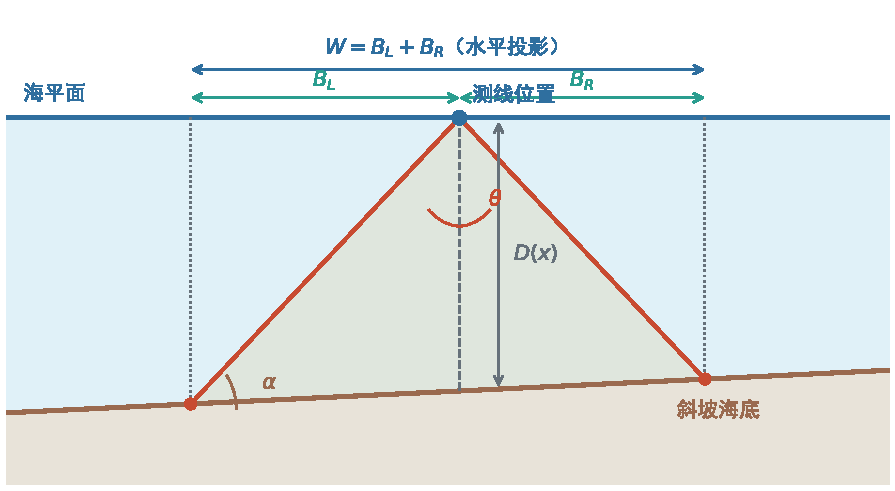
\includegraphics[width=0.82\textwidth]{../figures/q1/fig_q1_geometry.pdf}
  \caption{斜坡使左右半覆盖宽度不对称，而 $W=B_L+B_R$ 始终表示水平投影宽度}
  \label{fig:q1_geometry}
\end{figure}

\subsection{覆盖宽度模型}

声束边界同斜坡的交点决定条带两端。设半开角 $\phi=\theta/2$，由射线与斜坡直线的几何关系，左右半覆盖宽度的水平投影分别为

\begin{equation}
  B_L(x)=\frac{D(x)\sin\phi\cos\alpha}{\cos(\phi+\alpha)},\qquad
  B_R(x)=\frac{D(x)\sin\phi\cos\alpha}{\cos(\phi-\alpha)}.
  \label{eq:q1_half}
\end{equation}

分母中的 $\phi+\alpha$ 与 $\phi-\alpha$ 刻画斜坡对两侧声束的非对称作用。把两侧水平投影相加，可得条带覆盖宽度

\begin{equation}
  W(x)=B_L(x)+B_R(x)
      =D(x)\sin\phi\cos\alpha
      \left[\frac{1}{\cos(\phi+\alpha)}+\frac{1}{\cos(\phi-\alpha)}\right].
  \label{eq:q1_width}
\end{equation}

由于 $W(x)$ 与测线间距均为水平距离，二者可以直接用于覆盖判断。设相邻测线满足 $x_{i-1}<x_i$，水平间距为 $d_i=x_i-x_{i-1}$，则两条带在水平面上的代数重叠宽度为

\begin{equation}
  O_i=B_R(x_{i-1})+B_L(x_i)-d_i.
  \label{eq:q1_overlap_width}
\end{equation}

$O_i>0$ 表示重叠，$O_i<0$ 表示两条覆盖边界之间存在缺口。为与当前测线的覆盖能力比较，定义

\begin{equation}
  \eta_i=\frac{O_i}{W(x_i)}\times100\%.
  \label{eq:q1_overlap}
\end{equation}

该定义保留负值，因此同一指标既能表示冗余程度，也能直接识别漏测。

式~\eqref{eq:q1_overlap_width} 将前一条测线向浅水侧的覆盖范围与后一条测线向深水侧的覆盖范围相加，再扣除测线间距；以当前条带宽度归一化后，不同水深位置的重叠程度可以比较。

归一化分母取当前测线的条带宽度，使题面给定的各位置计算采用同一口径。代数重叠量保留负号：正值对应重复测量，负值的绝对值直接给出两条带之间的水平缺口，从而把冗余与漏测纳入同一判据。

\subsection{计算结果与规律}

取 $\theta=120^\circ$、$\alpha=1.5^\circ$、$D_0=70\text{ m}$，对题面给定的 9 个位置计算，结果见表~\ref{tab:q1}。

\begin{table}[H]
  \centering
  \caption{问题一各测线位置的水深、水平覆盖宽度与相邻重叠率}
  \label{tab:q1}
  \resizebox{\textwidth}{!}{%
    \begin{tabular}{lrrrrrrrrr}
      \toprule
      测线距中心点距离 / m & $-800$ & $-600$ & $-400$ & $-200$ & $0$ & $200$ & $400$ & $600$ & $800$ \\
      \midrule
      海水深度 / m & 90.95 & 85.71 & 80.47 & 75.24 & 70.00 & 64.76 & 59.53 & 54.29 & 49.05 \\
      覆盖宽度 / m & 315.71 & 297.53 & 279.35 & 261.17 & 242.99 & 224.81 & 206.63 & 188.45 & 170.27 \\
      重叠率 / \% & -- & 35.70 & 31.51 & 26.74 & 21.26 & 14.89 & 7.41 & $-1.53$ & $-12.36$ \\
      \bottomrule
    \end{tabular}%
  }
\end{table}

从深水侧向浅水侧移动时，水深由 $90.95\text{ m}$ 降至 $49.05\text{ m}$，覆盖宽度相应由 $315.71\text{ m}$ 单调降至 $170.27\text{ m}$。当相邻测线仍保持 $200\text{ m}$ 间距时，覆盖能力的下降不断消耗重叠余量：重叠率从 $35.70\%$ 降至 $-12.36\%$，并在 $x=600\text{ m}$ 处转为负值。这意味着固定间距同时造成深水侧冗余和浅水侧漏测，测线间距应随局部水深减小而收缩。图~\ref{fig:q1_result} 将这一因果链集中展示。

重叠率比覆盖宽度变化更敏感，因为它同时取决于前后条带边界与固定间距。当覆盖宽度接近 $200\text{ m}$ 时，水深继续下降会使正重叠迅速转为漏测，因此布线必须逐对检查相邻条带。

表格负责给出各位置的精确数值，图~\ref{fig:q1_result} 用于观察水深、覆盖宽度和重叠率的同步变化。浅水端的负重叠表明，按中心水深或平均宽度设置固定间距不能保证全域连续覆盖；后续布线应根据局部水深逐步收缩间距。

\begin{figure}[H]
  \centering
  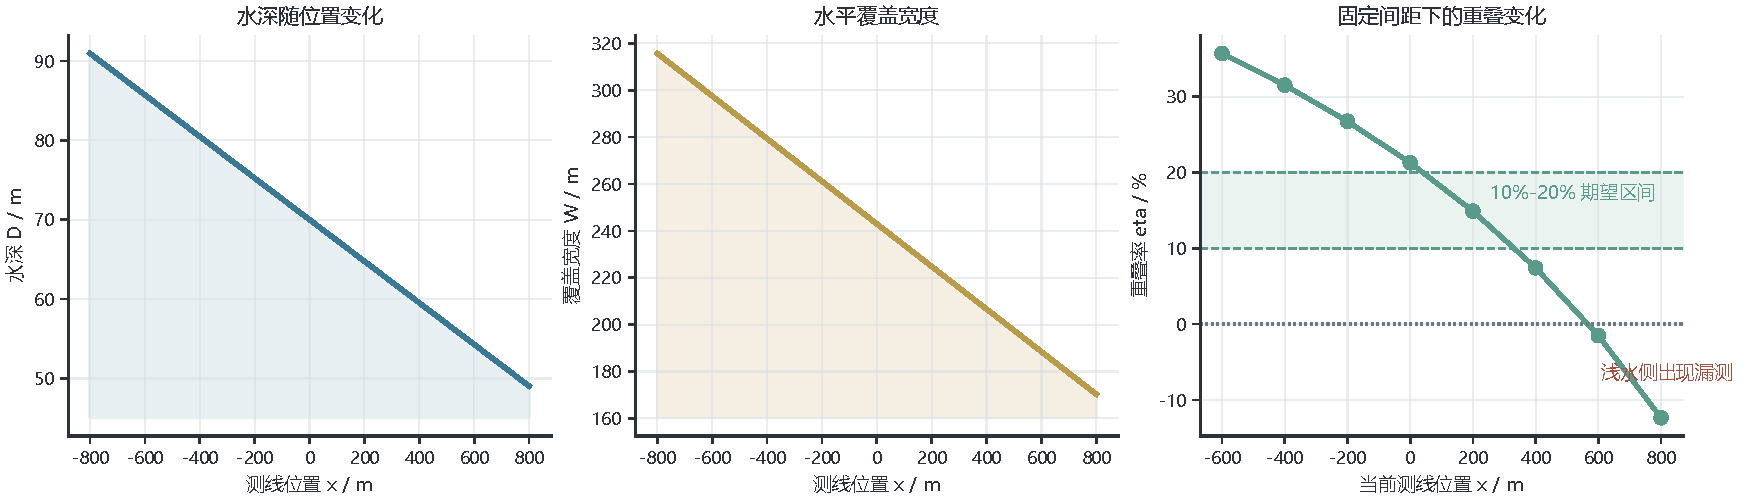
\includegraphics[width=1.0\textwidth]{../figures/q1/fig_q1_result.pdf}
  \caption{水深减小使水平覆盖宽度收缩，并推动固定间距下的重叠率由正转负}
  \label{fig:q1_result}
\end{figure}

\subsection{极限检验与敏感性分析}

当 $\alpha=0$ 时，式~\eqref{eq:q1_half} 退化为 $B_L=B_R=D\tan\phi$，进而有 $W=2D\tan(\theta/2)$、$\eta=1-d/W$，与题面平底公式一致。这一极限检验说明，水平投影口径在斜坡消失时能够无缝回到已知关系。

为比较两个几何参数的影响，在 $x=0$、$D_0=70\text{ m}$ 处分别扰动坡度与开角，结果见表~\ref{tab:sens}。

\begin{table}[H]
  \centering
  \caption{中心位置覆盖宽度对坡度和开角的单因素敏感性}
  \label{tab:sens}
  \begin{tabular}{lcccccc}
    \toprule
    $\alpha$ / $^\circ$（$\theta=120^\circ$） & 0.0 & 0.5 & 1.0 & 1.5 & 2.0 & 3.0 \\
    $W$ / m & 242.49 & 242.54 & 242.71 & 242.99 & 243.38 & 244.50 \\
    \midrule
    $\theta$ / $^\circ$（$\alpha=1.5^\circ$） & 100 & 110 & 120 & 130 & 140 & -- \\
    $W$ / m & 167.01 & 200.22 & 242.99 & 301.18 & 386.65 & -- \\
    \bottomrule
  \end{tabular}
\end{table}

坡度从 $0.0^\circ$ 增至 $3.0^\circ$ 时，覆盖宽度仅增加 $2.01\text{ m}$；开角从 $100^\circ$ 增至 $140^\circ$ 时，覆盖宽度则由 $167.01\text{ m}$ 增至 $386.65\text{ m}$。因此在本题小坡度范围内，开角决定基本覆盖尺度，水深变化决定沿程收缩趋势，坡度主要造成两侧覆盖不对称。

坡度对总宽度的影响较小，但仍会改变 $B_L$ 与 $B_R$ 的分配；后续模型因此保留等效坡度和左右半宽。

上述敏感性分析只比较单因素变化，不改变题面参数与主结果。它说明开角决定基本覆盖尺度，水深决定沿程收缩趋势，而坡度通过左右半宽的不对称影响相邻条带衔接。

本问解决了固定横断面内“覆盖多宽”的问题，但实际测线航向会同时改变船位水深和横断面坡度。下一问保留上述水平投影模型，仅把恒定坡度替换为航向坐标系中的等效坡度，由此将二维覆盖关系推广到三维海域。

\section{问题二的模型建立与求解}

\subsection{三维坡面到二维剖面的转化}

问题二把问题一的二维剖面推广到三维矩形海域。设测线方向与海底坡面法向在水平面上的投影夹角为 $\beta$，将坡面法向水平投影的正方向取为深水方向。多波束扫描平面垂直于测线方向，真正影响覆盖宽度的是坡度在该垂直剖面方向上的分量。因此定义垂直测线剖面内的等效坡度

\begin{equation}
  \alpha_{\mathrm{eff}}=\arctan\left(\tan\alpha\sin\beta\right).
  \label{eq:q2_alpha_eff}
\end{equation}

船位处水深由测线方向上的坡面高程变化确定。设测量船距海域中心点的距离为 $r$（海里），换算为 $s=1852r$ 米后，

\begin{equation}
  D(r,\beta)=D_0+s\tan\alpha\cos\beta.
  \label{eq:q2_depth}
\end{equation}

将问题一公式中的坡度替换为 $\alpha_{\mathrm{eff}}$、水深替换为 $D(r,\beta)$，得到覆盖宽度

\begin{equation}
  W(r,\beta)=D(r,\beta)\sin\phi\cos\alpha_{\mathrm{eff}}
  \left[\frac{1}{\cos(\phi+\alpha_{\mathrm{eff}})}+\frac{1}{\cos(\phi-\alpha_{\mathrm{eff}})}\right].
  \label{eq:q2_width}
\end{equation}

\subsection{求解与结果}

取 $\theta=120^\circ$、$\alpha=1.5^\circ$、$D_0=120\text{ m}$，对 $\beta=0^\circ,45^\circ,\dots,315^\circ$ 与 $r=0,0.3,\dots,2.1$ 海里代入式 \eqref{eq:q2_depth}--\eqref{eq:q2_width}，结果如表 3 和图 3 所示。

\begin{table}[H]
  \centering
  \caption{问题二覆盖宽度 / m}
  \label{tab:q2}
  \begin{tabular}{lrrrrrrrr}
    \toprule
    $\beta$ / $^\circ$ & 0 & 0.3 & 0.6 & 0.9 & 1.2 & 1.5 & 1.8 & 2.1 \\
    \midrule
    0   & 415.69 & 466.09 & 516.49 & 566.89 & 617.29 & 667.69 & 718.09 & 768.48 \\
    45  & 416.12 & 451.79 & 487.47 & 523.14 & 558.82 & 594.49 & 630.16 & 665.84 \\
    90  & 416.55 & 416.55 & 416.55 & 416.55 & 416.55 & 416.55 & 416.55 & 416.55 \\
    135 & 416.12 & 380.45 & 344.77 & 309.10 & 273.42 & 237.75 & 202.08 & 166.40 \\
    180 & 415.69 & 365.29 & 314.89 & 264.50 & 214.10 & 163.70 & 113.30 & 62.90  \\
    225 & 416.12 & 380.45 & 344.77 & 309.10 & 273.42 & 237.75 & 202.08 & 166.40 \\
    270 & 416.55 & 416.55 & 416.55 & 416.55 & 416.55 & 416.55 & 416.55 & 416.55 \\
    315 & 416.12 & 451.79 & 487.47 & 523.14 & 558.82 & 594.49 & 630.16 & 665.84 \\
    \bottomrule
  \end{tabular}
\end{table}

\begin{figure}[H]
  \centering
  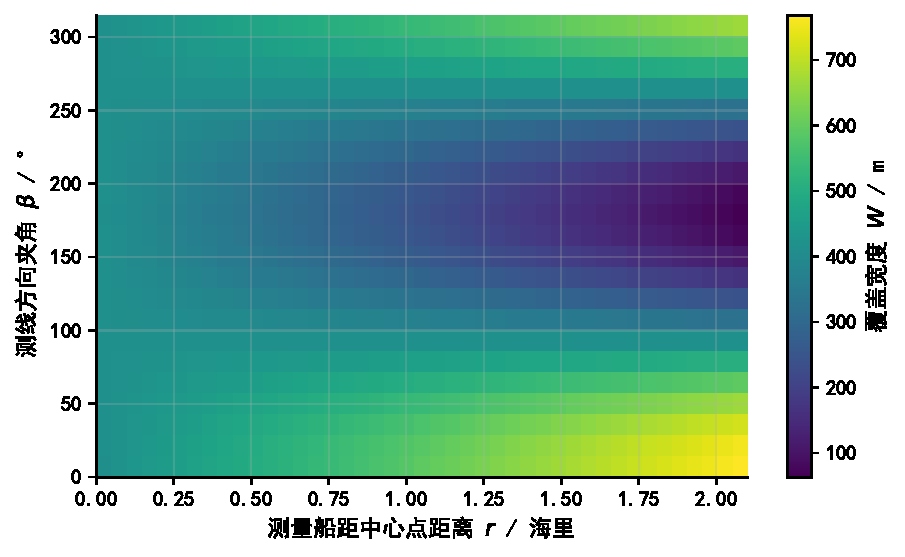
\includegraphics[width=0.78\textwidth]{../figures/q2/fig_q2_heatmap.pdf}
  \caption{覆盖宽度随测线方向夹角与船位距离的变化}
  \label{fig:q2_heatmap}
\end{figure}

\subsection{模型验证与本问结论}

当 $\beta=0^\circ$ 或 $180^\circ$ 时，测线方向沿坡面法向水平投影，垂直测线剖面沿等深线方向，$\alpha_{\mathrm{eff}}=0$，公式退化为平底公式 $W=2D\tan(\theta/2)$；当 $\beta=90^\circ$ 或 $270^\circ$ 时，船沿等深线运动，$D(r,\beta)=D_0$，覆盖宽度不随距离变化，与表 3 中该两行恒为 $416.55\text{ m}$ 一致。整体上覆盖宽度随水深增大而增大，$\beta=0^\circ$ 行随距离显著增大、$\beta=180^\circ$ 行随距离显著减小，符合物理直觉。

\section{问题三的模型建立与求解}

\subsection{优化模型的建立}

以矩形海域中心为原点建立水平坐标系，$x$ 向东为正（东侧为浅水），$y$ 向北为正。海域东西边界为 $x_{\min}=-3704\text{ m}$、$x_{\max}=3704\text{ m}$，南北边界为 $y_{\min}=-1852\text{ m}$、$y_{\max}=1852\text{ m}$（$1$ 海里 $=1852$ 米）。

由于海底为西深东浅的单一平面，等深线为南北向直线。测线沿等深线南北向布设时，每条线上的水深恒定，问题可降为一维布线。设第 $i$ 条测线坐标为 $x_i$，其两侧水平半覆盖宽度为

\begin{equation}
  B_W(x_i)=\frac{D(x_i)\sin\phi\cos\alpha}{\cos(\phi+\alpha)},\qquad
  B_E(x_i)=\frac{D(x_i)\sin\phi\cos\alpha}{\cos(\phi-\alpha)},
\end{equation}

其中 $D(x_i)=110-x_i\tan\alpha$。相邻条带的代数重叠宽度与重叠率为

\begin{equation}
  O_i=B_E(x_{i-1})+B_W(x_i)-(x_i-x_{i-1}),\qquad
  \eta_i=\frac{O_i}{B_W(x_i)+B_E(x_i)}\times100\%.
\end{equation}

为保证完全覆盖，首条测线西侧覆盖边界应覆盖西边界，末条测线东侧覆盖边界应覆盖东边界：

\begin{equation}
  x_1-B_W(x_1)\le x_{\min},\qquad
  x_n+B_E(x_n)\ge x_{\max}.
\end{equation}

相邻重叠率应满足 $10\%\le\eta_i\le20\%$。每条测线贯穿矩形，长度均为 $y_{\max}-y_{\min}=3704\text{ m}$，故总长度最小等价于测线数最少。问题三转化为

\begin{equation}
  \min n,\qquad \text{s.t.}\quad
  \begin{aligned}[t]
    &10\%\le\eta_i\le20\%,\quad i=2,\dots,n,\\
    &x_1-B_W(x_1)\le x_{\min},\\
    &x_n+B_E(x_n)\ge x_{\max}.
  \end{aligned}
  \label{eq:q3_opt}
\end{equation}

\subsection{贪心递推求解}

为最小化测线数，第一步将首条测线尽可能向东放置，同时令其西侧覆盖边界正好覆盖西边界，即求解 $x_1-B_W(x_1)=x_{\min}$。此后每一步在保证与前一条测线之间无漏测的前提下取最大可行间距，即令重叠率取约束下限 $\eta_i=10\%$，用二分法递推 $x_i$，直至末条测线覆盖东边界。

\subsection{求解结果}

程序得到推荐方案：测线方向为南北向、平行等深线，共 $34$ 条；每条测线长 $2$ 海里，总长度 $68.00$ 海里，即 $125936.00\text{ m}$。布设俯视图见图 4，相邻间距与重叠率校验见图 5。

\begin{figure}[H]
  \centering
  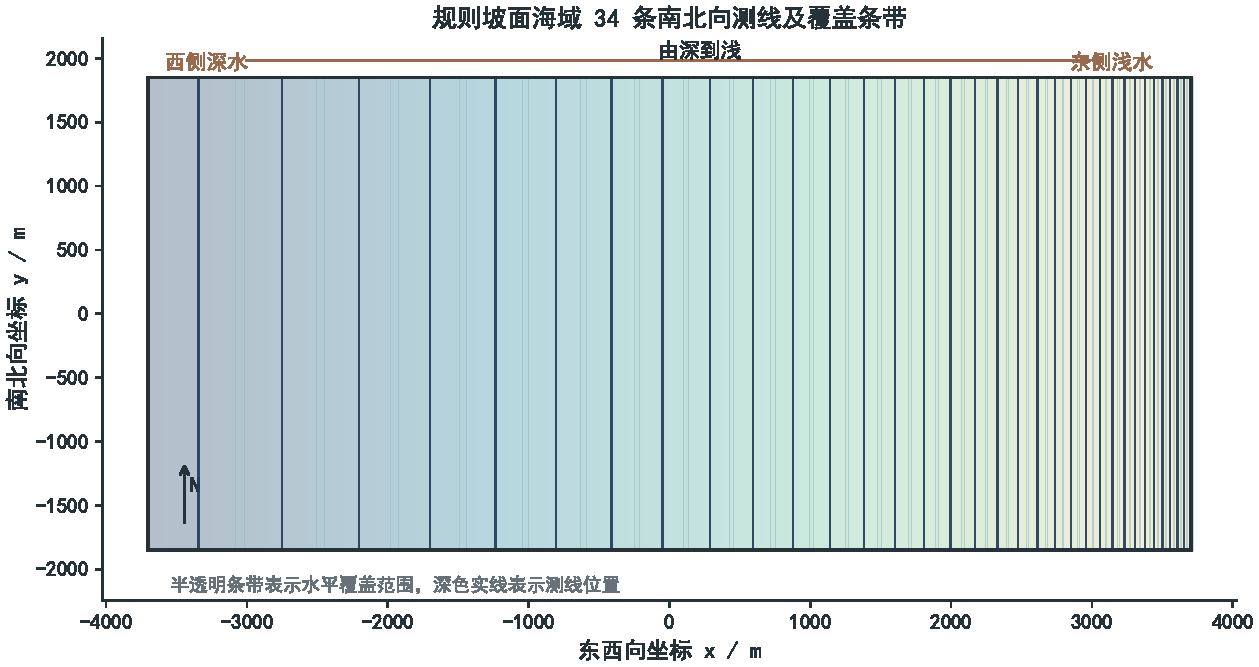
\includegraphics[width=0.9\textwidth]{../figures/q3/fig_q3_layout.pdf}
  \caption{34 条南北向测线在矩形海域内的布设}
  \label{fig:q3_layout}
\end{figure}

\begin{figure}[H]
  \centering
  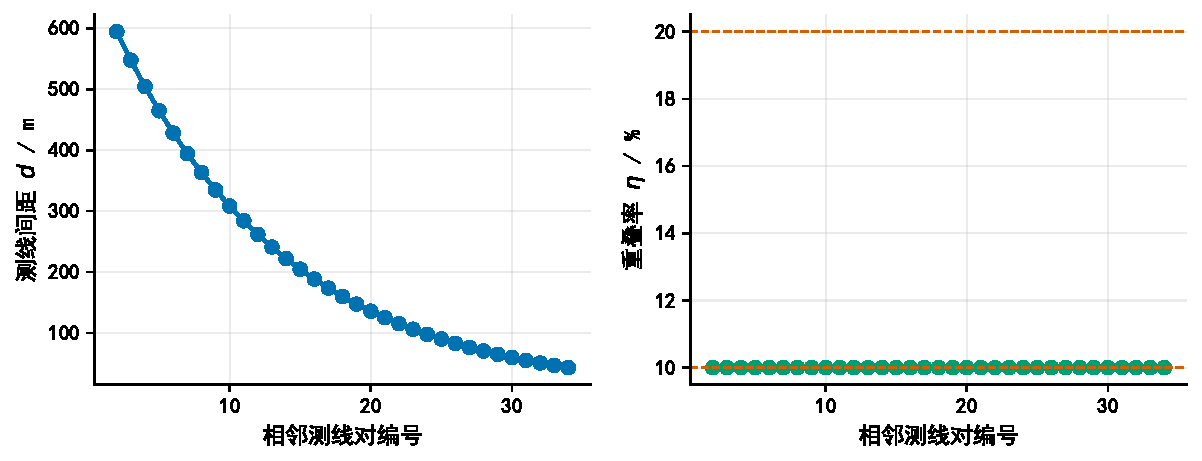
\includegraphics[width=0.95\textwidth]{../figures/q3/fig_q3_spacing.pdf}
  \caption{相邻测线间距与重叠率随测线对编号的变化}
  \label{fig:q3_spacing}
\end{figure}

\subsection{模型验证与本问结论}

完全覆盖检验表明，首条测线西覆盖边界为 $-3704.00\text{ m}$、末条测线东覆盖边界为 $3719.41\text{ m}$，东西方向无漏测；逐对复算 $33$ 个相邻重叠率均为 $10.00\%$，满足 $10\%\sim20\%$。最小条数检验表明，若少一条测线，在同样取最大可行间距的情况下最东覆盖边界仅为 $3678.24\text{ m}$，距东边界仍有 $25.76\text{ m}$ 缺口，因此 $33$ 条不可行。故该方案在所选方向与布线规则下测线数已不可再减少。

\section{问题四：真实海域测线设计}

\subsection{问题分析与评价标准}

真实海域在东西、南北两个方向均有起伏，同一条长测线上的水深和横向坡度不再恒定。若仍按全域最不利位置确定间距，局部浅水会限制整条测线，造成深水区冗余；若使用平均水深，又可能遗漏局部浅水区。因此，本问保留南北向递推，将海域分条后用局部梯度计算覆盖边界。

问题三把 $10\%\sim20\%$ 重叠率作为规则斜坡上的相邻测线约束；问题四以全区域覆盖为首要目标，以总测线长度和重叠率超过 $20\%$ 的累计长度评价候选方案。真实非均匀地形中，局部重叠率可能低于 $10\%$ 或高于 $20\%$，方案有效性由原始网格回代后的覆盖完整性与累计指标共同判断。局部超限仍需披露，并用于识别冗余集中区域。

两问的评价口径由此分开：问题三要求每对规则条带满足区间约束，问题四比较在全覆盖前提下的长度与累计冗余。前者输出固定航向下的最短可行线数，后者输出若干分条尺度的指标表，并区分题面数学指标最优方案与包含组织成本判断的工程折中方案。

\subsection{数据预处理}

附件包含 $201\times251$ 个规则网格点，横坐标为 $0\sim4$ 海里，纵坐标为 $0\sim5$ 海里，步长均为 $0.02$ 海里，共 $50451$ 个水深值。检查确认坐标单调、网格维度匹配且水深无缺失；水深范围为 $20.00\sim197.20\text{ m}$，平均值为 $62.54\text{ m}$。计算时按 $1$ 海里 $=1852$ m 统一转换坐标，测线位置不落在原网格列上时，仅沿东西方向线性插值水深与梯度，覆盖评价仍返回原始网格。

预处理还统一了矩阵行列与空间方向：水深矩阵的列对应东西坐标，行对应南北坐标，西侧为深水区、东侧为浅水区。梯度计算在米制坐标中进行，防止把“每海里水深变化”直接当作无量纲坡度。原数据无需缺失值填补或异常值替换，因此不改变任何附件水深值。

图~\ref{fig:q4_bathymetry_surface} 显示海底总体西深东浅，南北向局部起伏使单一平面坡近似不足。

\begin{figure}[H]
  \centering
  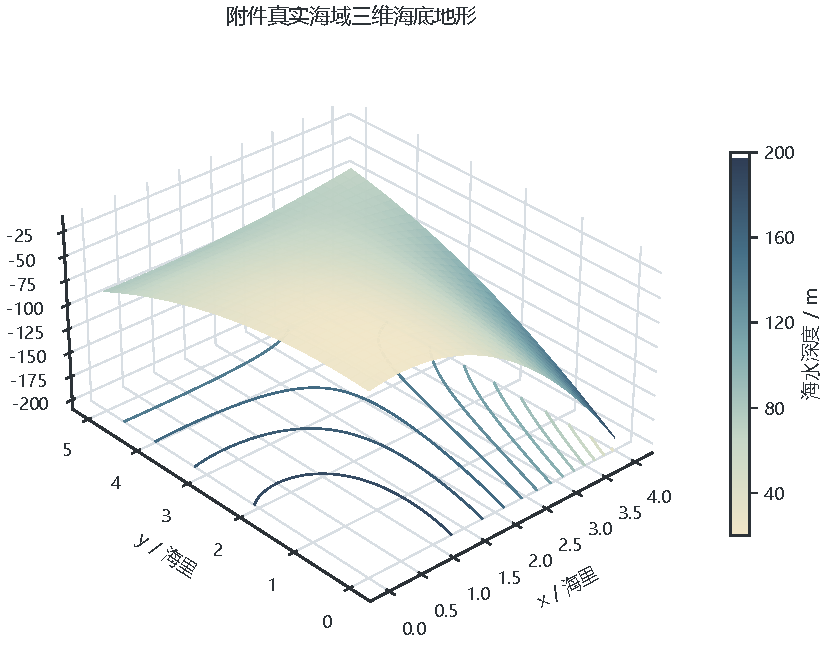
\includegraphics[width=0.8\textwidth]{../figures/q4/fig_q4_bathymetry_surface.pdf}
  \caption{真实海底总体西深东浅，南北向局部起伏要求测线按区域适应地形}
  \label{fig:q4_bathymetry_surface}
\end{figure}

\subsection{局部坡度与覆盖模型}

南北向测线的扫描剖面沿东西方向展开，左右覆盖边界主要由东西向梯度 $g_x=\partial D/\partial x$ 决定。在网格点 $(x,y)$ 邻域内，将海底近似为

\begin{equation}
  D(x+u,y)\approx D(x,y)+g_x(x,y)u.
\end{equation}

设换能器半开角为 $\phi$，声束边界与局部线性海底相交后，两侧水平半覆盖宽度为

\begin{equation}
  B_W(x,y)=\frac{D(x,y)}{\cot\phi+g_x(x,y)},\qquad
  B_E(x,y)=\frac{D(x,y)}{\cot\phi-g_x(x,y)}.
  \label{eq:q4_half}
\end{equation}

条带水平宽度为 $W_h=B_W+B_E$。对相邻测线 $x_i<x_{i+1}$，同一纵向位置 $y$ 上的局部重叠率为

\begin{equation}
  \eta_i(y)=\frac{B_E(x_i,y)+B_W(x_{i+1},y)-(x_{i+1}-x_i)}{W_h(x_{i+1},y)}\times100\%.
\end{equation}

网格点 $(x,y)$ 被第 $i$ 条测线覆盖，当且仅当
$x_i-B_W(x_i,y)\le x\le x_i+B_E(x_i,y)$。南北向梯度通过同一线段不同 $y$ 位置的水深与 $g_x$ 间接进入逐行计算。局部线性化只在网格邻域和短距离声束作用范围内有效，坡度突变区的误差由原网格回代进一步检查。

这里不用完整梯度模长替代 $g_x$。完整梯度同时包含沿航向的南北分量，而覆盖边界位于垂直航向的东西剖面；直接使用模长会把沿程水深变化重复计入横向坡度。南北起伏仍通过逐行变化的 $D(x,y)$ 和 $g_x(x,y)$ 进入每个覆盖截面。

\subsection{分条递推与候选方案生成}

将海域沿南北方向划分为水平条带。每个条带内，首条线取能够覆盖所有采样行西边界的最东位置；随后按问题三的最大允许间距向东递推，并以带内最不利位置保证相邻条带无间隙，直至覆盖东边界。不同条带独立生成测线段，合并后形成全域方案。图~\ref{fig:q4_contour} 展示 $0.50$ 海里方案的等深线、条带边界和测线位置。

“最不利位置”指使西边界覆盖或相邻条带衔接最紧的采样行，而非带内平均水深位置。以该位置递推会在其他行产生一定冗余，但可避免平均值掩盖局部浅水缺口。各条带分别求首线和后续线坐标，算法结构与问题三一致，仅将单一覆盖宽度替换为带内逐行覆盖边界。

\begin{figure}[H]
  \centering
  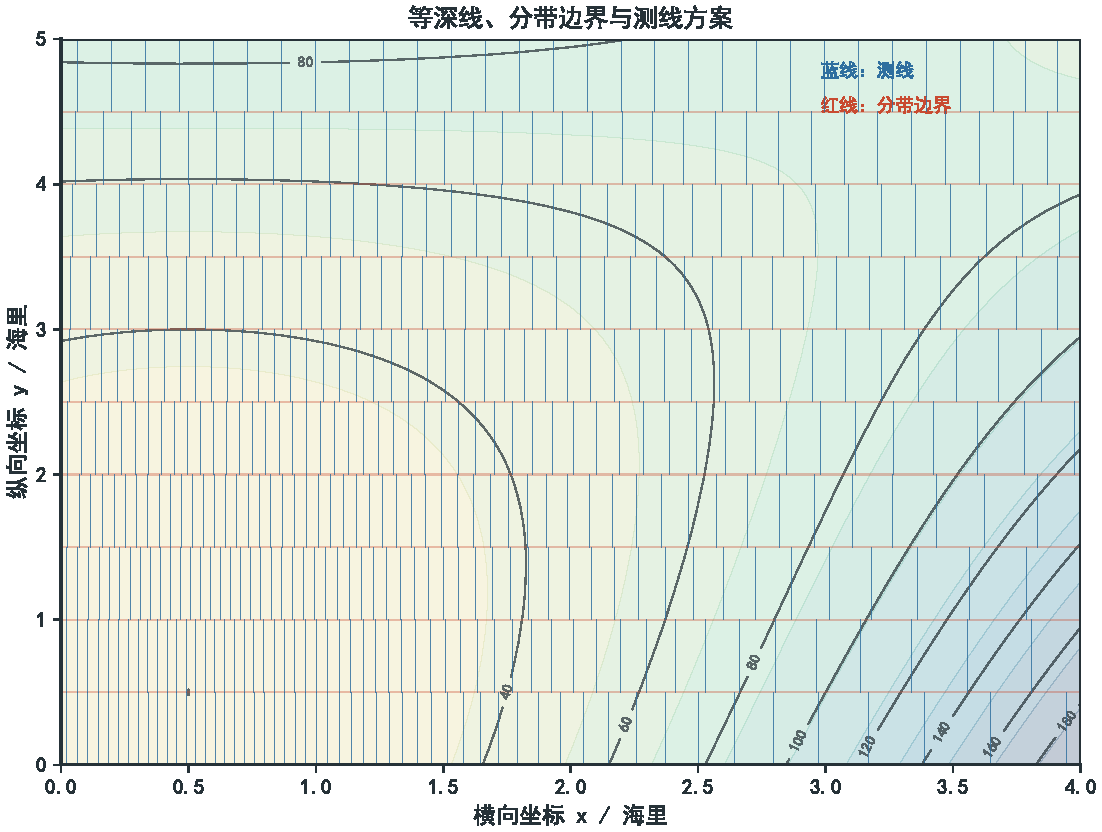
\includegraphics[width=0.8\textwidth]{../figures/q4/fig_q4_contour_route_overlay.pdf}
  \caption{$0.50$ 海里分条方案根据局部等深线调整测线位置，并覆盖东西边界}
  \label{fig:q4_contour}
\end{figure}

取 $5.00$、$1.00$、$0.50$ 和 $0.25$ 海里四种条带高度生成候选方案。四组计算保持换能器开角、测线方向、覆盖公式和网格评价方法不变；条带越短，带内最不利条件越接近局部地形，但线段数量和转场组织复杂度随之增加。

$5.00$ 海里方案把全域视为一个条带，提供不分条时的基准；其余三种尺度逐步细化南北方向的条带。候选集用于观察局部适应能力与线段组织成本的变化，不预先给任何方案附加综合权重。

\subsection{原始网格回代及指标计算}

全部候选测线生成后，返回原始 $201\times251$ 网格逐点计算覆盖和重叠。评价指标在比较结果前统一定义：总测线长度为全部实际测量线段长度之和，不含转场、调头和连接航程；漏测率为未被任何条带覆盖的原始网格点比例；平均重叠率和最大重叠率由原网格各相邻条带的 $\eta_i(y)$ 统计；超 $20\%$ 重叠长度为满足 $\eta_i(y)>20\%$ 的区段累计长度。边界覆盖、带内相邻关系和全网格复算构成三层检查。

三层检查的对象不同：边界检查确认各带首末覆盖范围封闭，带内检查确认相邻测线之间没有水平间隙，全网格检查统计离散地形上的漏测与局部重叠。若某层失败，可分别定位为边界放置、递推间距或局部线性近似问题，而不以单一汇总指标掩盖原因。

\subsection{候选方案比较与最终选择}

四种分条尺度的回代结果见表~\ref{tab:q4}。

\begin{table}[H]
  \centering
  \caption{不同分条尺度下的覆盖、冗余与线段组织成本}
  \label{tab:q4}
  \resizebox{\textwidth}{!}{%
    \begin{tabular}{lccccc}
      \toprule
      方案 & 线段数 & 总长度 / m & 漏测率 / \% & 超 $20\%$ 重叠长度 / m & 最大重叠率 / \% \\
      \midrule
      全域 $5.00$ NM & 60  & 555600.00 & 0.00 & 276877.69 & 76.42 \\
      $1.00$ NM      & 240 & 444480.00 & 0.00 & 51525.55  & 45.86 \\
      $0.50$ NM      & 461 & 426886.00 & 0.00 & 5481.92   & 49.01 \\
      $0.25$ NM      & 897 & 415311.00 & 0.00 & 2742.38   & 46.07 \\
      \bottomrule
    \end{tabular}%
  }
\end{table}

四种方案的漏测率均为 $0.00\%$。分条从 $5.00$ 海里细化到 $0.25$ 海里时，总长度由 $555.600$ km 降至 $415.311$ km，超 $20\%$ 重叠长度由 $276877.69$ m 降至 $2742.38$ m，线段数则由 60 增至 897。细分减弱了全带最不利水深的限制，同时提高了作业组织成本。

按题面直接要求的总长度、漏测率和超重叠长度，$0.25$ 海里方案是四个候选方案中的数学指标最优方案。若考虑题面未计入的转场与调头负担，$0.50$ 海里方案将线段数由 897 降至 461，总长为 $426.886$ km，超重叠长度为 $5481.92$ m，平均相邻重叠率为 $4.66\%$，可作为工程折中。该推荐不等同于单项数学指标的唯一最优解。

从 $0.50$ 海里进一步细化至 $0.25$ 海里，总长度由 $426.886$ km 降至 $415.311$ km，超重叠长度由 $5481.92$ m 降至 $2742.38$ m，但线段数由 461 增至 897。题面未给出船速、转弯半径或单次调头耗时，无法把组织成本折算为统一费用；因此表格保留原始指标，工程推荐只作为有条件的折中判断。

\subsection{局部重叠超限及适用边界}

$0.50$ 海里方案回代后的覆盖率为 $100\%$，但最大局部重叠率为 $49.01\%$，超限主要集中在局部坡度变化较大及各条带独立递推的边界附近。平均重叠率较低，源于多数区段按覆盖完整性控制间距，而少量极端位置贡献了较高最大值；因此平均值、累计超限长度和局部最大值需同时报告。

分条边界两侧的测线由相邻条带分别递推，地形条件和首线位置可能不同，因而容易出现局部覆盖叠加；坡度突变又会使左右半宽在短距离内快速变化。两类因素增加局部最大值，但原网格回代显示其未造成覆盖缺口。超限累计长度用于衡量这部分冗余的空间规模。

当前方案保证原始网格点无漏测，并以累计长度衡量局部冗余，未要求每一点均满足 $10\%\sim20\%$。若将 $20\%$ 设为逐点硬约束，需要重新调整条带边界或局部测线位置；坡度突变、网格间细尺度地形及声速分层也会降低局部线性模型的精度。上述因素限定了方案作为测前规划的适用范围。

原网格漏测率 $0.00\%$ 只说明给定采样点均被覆盖，不能排除采样间隔内存在未解析的细小地形突变。实际作业应结合实时水深、姿态和声速信息复核覆盖边界，并在高坡度区和分条接缝附近预留更高安全重叠率。

\section{敏感性分析}

\subsection{问题一覆盖宽度对坡度与开角的敏感性}

为考察几何模型对关键输入参数的敏感程度，在 $x=0$、$D_0=70\text{ m}$ 处分别单独扰动坡度 $\alpha$ 与换能器开角 $\theta$，覆盖宽度变化如表 5 所示。

\begin{table}[H]
  \centering
  \caption{问题一覆盖宽度对坡度与开角的单因素敏感性}
  \label{tab:sens}
  \begin{tabular}{lcccccc}
    \toprule
    $\alpha$ / $^\circ$（$\theta=120^\circ$） & 0.0 & 0.5 & 1.0 & 1.5 & 2.0 & 3.0 \\
    $W$ / m & 242.49 & 242.54 & 242.71 & 242.99 & 243.38 & 244.50 \\
    \midrule
    $\theta$ / $^\circ$（$\alpha=1.5^\circ$） & 100 & 110 & 120 & 130 & 140 & -- \\
    $W$ / m & 167.01 & 200.22 & 242.99 & 301.18 & 386.65 & -- \\
    \bottomrule
  \end{tabular}
\end{table}

由表 5 可知，覆盖宽度对坡度 $\alpha$ 的敏感程度较低，在 $0.0^\circ\sim3.0^\circ$ 范围内 $W$ 仅变化约 $2.01\text{ m}$；而覆盖宽度对开角 $\theta$ 明显更敏感，$\theta$ 从 $100^\circ$ 增至 $140^\circ$ 时 $W$ 由 $167.01\text{ m}$ 增至 $386.65\text{ m}$。这说明在本题给定的小坡度范围内，可把坡度近似作为弱影响因素，而换能器开角是决定覆盖宽度的主要参数。

\subsection{问题三最小测线数的约束敏感性}

问题三的递推求解取重叠率下限 $10\%$ 作为每步最大间距条件，方案恰好落在约束边界上。若在相同布线方向下减少一条测线，最东覆盖边界由 $3719.41\text{ m}$ 降至 $3678.24\text{ m}$，出现 $25.76\text{ m}$ 缺口。该结果表明 $34$ 条测线对该 $10\%\sim20\%$ 重叠率约束是紧的，方案对重叠率下限的变化较为敏感。

\subsection{问题四分带粒度的敏感性}

问题四的分带高度从 $5.00$ 海里细化到 $0.25$ 海里时，测线总长度由 $555600.00\text{ m}$ 降至 $415311.00\text{ m}$，超 $20\%$ 重叠长度由 $276877.69\text{ m}$ 降至 $2742.38\text{ m}$，漏测率始终为 $0.00\%$。可见分带粒度对冗余控制影响显著；推荐 $0.50$ 海里方案是在三项指标与线段数、转场成本之间的折中选择。

\section{模型评价与推广}

\subsection{模型优点}

\begin{enumerate}
  \item 覆盖宽度与重叠率全程使用“水平投影”口径，可与水平测线间距直接比较，避免了斜坡情形下坡面长度与水平距离混用的问题；
  \item 问题一、二均为确定性解析几何模型，参数可解释、结果可复算，并在 $\alpha=0$ 或 $\beta=0^\circ,180^\circ$ 等特殊情形下退化为平底公式，模型正确性有明确检验；
  \item 问题三的贪心递推针对单一平面坡面可证明在当前方向下测线数不可再减少，结果具有可解释的最优性；
  \item 问题四采用分带策略并保留网格覆盖仿真，能够处理真实地形下的深浅差异，方案与题目三项指标直接对应。
\end{enumerate}

\subsection{模型不足}

\begin{enumerate}
  \item 问题一至问题三假设海底为理想平面斜坡、声波沿直线传播，未考虑真实声速剖面、折射和复杂地形；
  \item 问题四仅统计测量线段长度，未计入不同线段之间的转场、调头和航行连接成本，可能低估实际作业代价；
  \item 分带边界处各带独立布线的覆盖近似会引入少量重叠误差，局部最大相邻重叠率仍达 $49.01\%$；
  \item 问题四未进行随机扰动或全局优化，所得为当前分带与递推规则下的较优方案，而非严格全局最优。
\end{enumerate}

\subsection{模型推广}

模型可推广到一般起伏海底：保留“水平投影覆盖宽度 + 相邻重叠率”的评价框架，将平面坡度替换为局部梯度估计即可用于非规则地形。若进一步引入声速分层，可在射线追踪中修正声线曲率；若考虑船舶转弯与多船协同，可把分带递推扩展为带转场代价的路径优化问题。


\newpage
\referencescn
\newpage
\appendixcn

\end{document}
